\documentclass[11pt]{article}
\usepackage[utf8]{inputenc}
\usepackage[T1]{fontenc}
\usepackage{amsmath}
\usepackage{multicol}
\usepackage{geometry}
\usepackage{tikz}
\usetikzlibrary{shapes.geometric, arrows.meta}
\usepackage{enumitem}
\usepackage{xcolor}
\usepackage{titlesec}

% Configurações de layout
\geometry{a4paper, left=1cm, right=1cm, top=0.5cm, bottom=1.2cm}
\setlength{\columnseprule}{0.4pt}
\setlength{\baselineskip}{1.0\baselineskip}

% Cores para títulos
\titleformat{\section}{\normalfont\Large\bfseries\color{blue}}{\thesection}{1em}{}
\titleformat{\subsection}{\normalfont\large\bfseries\color{red}}{\thesubsection}{1em}{}
\titleformat{\subsubsection}{\normalfont\normalsize\bfseries\color{black}}{\thesubsubsection}{1em}{}

\title{\textcolor{blue}{Função do 2º Grau: Parábolas e Aplicações}}
\author{Professor: Jefferson}
\date{}

\begin{document}

\maketitle
\vspace{-1cm}

\begin{center}
\large{Nome: \underline{\hspace{8cm}} \quad Turma: \underline{\hspace{3cm}}}
\end{center}

\begin{multicols}{2}

\section*{1. Conceito}
Uma função do 2º grau (ou quadrática) é expressa por:
\[
f(x) = ax^2 + bx + c \quad \text{ou} \quad y = ax^2 + bx + c
\]
onde:
\begin{itemize}
    \item $a$, $b$, $c$ são coeficientes reais ($a \neq 0$)
    \item $x$ é a variável independente
    \item O gráfico é sempre uma \textbf{parábola}
\end{itemize}

\subsection*{Exemplos}
\begin{itemize}
    \item $f(x) = x^2 - 4x + 3$ \quad ($a=1$, $b=-4$, $c=3$)
    \item $y = -2x^2 + 8x$ \quad ($a=-2$, $b=8$, $c=0$)
    \item $f(x) = \frac{1}{2}x^2 + 1$ \quad ($a=\frac{1}{2}$, $b=0$, $c=1$)
\end{itemize}

\section*{2. Gráfico: Parábola}
Características principais:
\begin{itemize}
    \item \textbf{Concavidade}: Para cima ($a>0$) ou para baixo ($a<0$)
    \item \textbf{Vértice}: Ponto de máximo/mínimo
    \item \textbf{Eixo de simetria}: Linha vertical que passa pelo vértice
\end{itemize}

\begin{center}
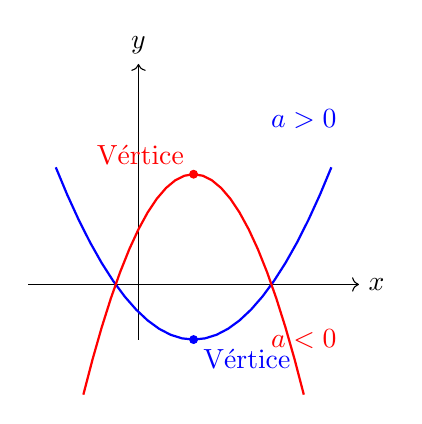
\begin{tikzpicture}[scale=0.7]
    % Eixos
    \draw[->] (-2,0) -- (4,0) node[right]{$x$};
    \draw[->] (0,-1) -- (0,4) node[above]{$y$};
    % Parábolas
    \draw[blue, thick, domain=-1.5:3.5] plot (\x, {0.5*\x*\x - \x - 0.5});
    \node[blue] at (3,3) {$a>0$};
    \draw[red, thick, domain=-1:3] plot (\x, {-\x*\x + 2*\x + 1});
    \node[red] at (3,-1) {$a<0$};
    % Vértices
    \filldraw[blue] (1,-1) circle (2pt) node[below right]{Vértice};
    \filldraw[red] (1,2) circle (2pt) node[above left]{Vértice};
\end{tikzpicture}
\end{center}

\section*{3. Concavidade}
\begin{itemize}
    \item \textbf{Para cima} ($a > 0$): Concavidade voltada para cima.
    \item \textbf{Para baixo} ($a < 0$): Concavidade voltada para baixo.
\end{itemize}

\begin{center}
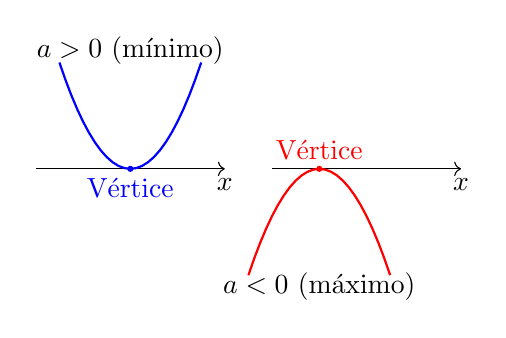
\begin{tikzpicture}[scale=0.6]
    % a > 0
    \draw[->] (-2,0) -- (2,0) node[below]{$x$};
    \draw[blue, thick, domain=-1.5:1.5] plot (\x, \x*\x);
    \filldraw[blue] (0,0) circle (1.5pt) node[below]{Vértice};
    \node at (0,2.5) {$a>0$ (mínimo)};
    % a < 0 (agora tangenciando o eixo x)
    \draw[->] (3,0) -- (7,0) node[below]{$x$};
    \draw[red, thick, domain=2.5:5.5] plot (\x, {-(\x-4)*(\x-4)}); % Equação modificada
    \filldraw[red] (4,0) circle (1.5pt) node[above]{Vértice};
    \node at (4,-2.5) {$a<0$ (máximo)};
\end{tikzpicture}
\end{center}

\section*{4. Zeros da Função (Raízes)}
Soluções da equação $ax^2 + bx + c = 0$:
\[
x = \frac{-b \pm \sqrt{\Delta}}{2a}
\]
\begin{itemize}
    \item $\Delta > 0$: Duas raízes reais distintas
    \item $\Delta = 0$: Uma raiz real dupla
    \item $\Delta < 0$: Nenhuma raiz real
\end{itemize}

\begin{center}
\begin{tikzpicture}[scale=0.6]
    % Delta > 0
    \draw[->] (-2,0) -- (2,0);
    \draw[blue, thick, domain=-1.3:1.3] plot (\x, {\x*\x - 0.5});
    \filldraw (-0.707,0) circle (1.5pt);
    \filldraw (0.707,0) circle (1.5pt);
    \node at (0,-2) {$\Delta > 0$};
    % Delta = 0
    \draw[->] (3,0) -- (7,0);
    \draw[red, thick, domain=4.3:5.7] plot (\x, {(\x-5)*(\x-5)});
    \filldraw (5,0) circle (1.5pt);
    \node at (5,-2) {$\Delta = 0$};
    % Delta < 0
    \draw[->] (8,0) -- (12,0);
    \draw[green, thick, domain=9:11] plot (\x, {(\x-10)*(\x-10)+1});
    \node at (10,-2) {$\Delta < 0$};
\end{tikzpicture}
\end{center}

\begin{center}
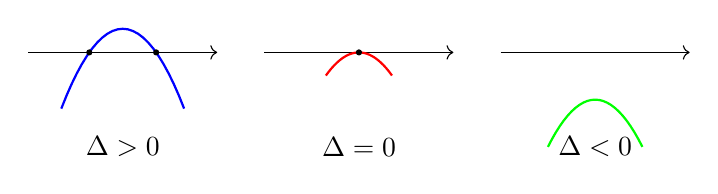
\begin{tikzpicture}[scale=0.6]
    % Delta > 0 (concavidade para baixo)
    \draw[->] (-2,0) -- (2,0);
    \draw[blue, thick, domain=-1.3:1.3] plot (\x, {-\x*\x + 0.5});
    \filldraw (-0.707,0) circle (1.5pt);
    \filldraw (0.707,0) circle (1.5pt);
    \node at (0,-2) {$\Delta > 0$};
    
    % Delta = 0 (concavidade para baixo)
    \draw[->] (3,0) -- (7,0);
    \draw[red, thick, domain=4.3:5.7] plot (\x, {-(\x-5)*(\x-5)});
    \filldraw (5,0) circle (1.5pt);
    \node at (5,-2) {$\Delta = 0$};
    
    % Delta < 0 (concavidade para baixo)
    \draw[->] (8,0) -- (12,0);
    \draw[green, thick, domain=9:11] plot (\x, {-(\x-10)*(\x-10)-1});
    \node at (10,-2) {$\Delta < 0$};
\end{tikzpicture}
\end{center}

\section*{5. Vértice da Parábola}
Coordenadas do vértice ($V$):
\[
V\left( -\frac{b}{2a}, -\frac{\Delta}{4a} \right)
\]
onde $\Delta = b^2 - 4ac$.

\subsection*{Exemplo}
Para $f(x) = x^2 - 6x + 5$:
\[
V\left( -\frac{-6}{2\cdot1}, -\frac{16}{4\cdot1} \right) = (3, -4)
\]

\section*{6. Estudo do Sinal}
\begin{itemize}
    \item Depende do sinal de $a$ e do $\Delta$
    \item Regra prática:
    \begin{enumerate}
        \item Identifique as raízes (se existirem)
        \item Observe a concavidade
        \item Faça o "varal" de sinais
    \end{enumerate}
\end{itemize}

\begin{center}
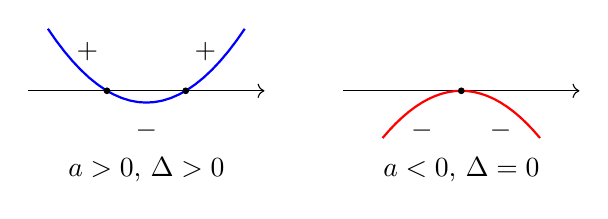
\begin{tikzpicture}[scale=0.5]
    % Caso a>0, Delta>0
    \draw[->] (-1,0) -- (5,0);
    \draw[blue, thick, domain=-0.5:4.5] plot (\x, {0.3*(\x-1)*(\x-3)});
    \filldraw (1,0) circle (2pt);
    \filldraw (3,0) circle (2pt);
    \node at (0.5,1) {$+$};
    \node at (2,-1) {$-$};
    \node at (3.5,1) {$+$};
    \node at (2,-2) {$a>0$, $\Delta>0$};
    
    % Caso a<0, Delta=0
    \draw[->] (7,0) -- (13,0);
    \draw[red, thick, domain=8:12] plot (\x, {-0.3*(\x-10)*(\x-10)});
    \filldraw (10,0) circle (2pt);
    \node at (9,-1) {$-$};
    \node at (11,-1) {$-$};
    \node at (10,-2) {$a<0$, $\Delta=0$};
\end{tikzpicture}
\end{center}

\section*{2. Gráfico: Parábola}
Características principais:
\begin{itemize}
    \item \textbf{Concavidade}: Para cima ($a>0$) ou para baixo ($a<0$)
    \item \textbf{Eixo de simetria}: Linha vertical que divide a parábola em duas partes simétricas
\end{itemize}

\section*{3. Zeros da Função (Raízes)}
Soluções da equação $ax^2 + bx + c = 0$:
\[
x = \frac{-b \pm \sqrt{b^2 - 4ac}}{2a}
\]
\begin{itemize}
    \item $\Delta > 0$: Duas raízes reais distintas
    \item $\Delta = 0$: Uma raiz real dupla
    \item $\Delta < 0$: Nenhuma raiz real
\end{itemize}

\section*{4. Exercícios}

\begin{enumerate}
    \item Dada $f(x) = x^2 - 5x + 6$, determine:
    \begin{enumerate}[label=\alph*)]
        \item Os coeficientes $a$, $b$, $c$
        \item As raízes da função
        \item O valor de $f(0)$
        \item O valor de $f(1)$
        \item O valor de $f(2)$
    \end{enumerate}
    
    \item Classifique a concavidade:
    \begin{enumerate}[label=\alph*)]
        \item $y = 3x^2 - 2x + 1$
        \item $f(x) = -x^2 + 4$
        \item $y = \frac{1}{2}x^2 - 3x$
        \item $f(x) = -3x^2 + x - 2$
        \item $y = 0.5x^2 + 1$
    \end{enumerate}
    
    \item Calcule $\Delta$ para:
    \begin{enumerate}[label=\alph*)]
        \item $x^2 - 6x + 9 = 0$
        \item $2x^2 + x - 3 = 0$
        \item $x^2 + 4x + 5 = 0$
        \item $-3x^2 + 7x - 2 = 0$
        \item $5x^2 - 10x + 5 = 0$
    \end{enumerate}
    
    \item Resolva as equações:
    \begin{enumerate}[label=\alph*)]
        \item $x^2 - 5x + 6 = 0$
        \item $2x^2 + 3x - 2 = 0$
        \item $x^2 - 4x + 4 = 0$
        \item $3x^2 - x - 2 = 0$
        \item $-x^2 + 2x - 1 = 0$
    \end{enumerate}
\end{enumerate}

\begin{enumerate}\setcounter{enumi}{4}
    \item Para cada função, determine:
    \begin{enumerate}[label=\alph*)]
        \item As raízes de $f(x) = x^2 - 4x + 3$
        \item As raízes de $f(x) = -x^2 + 2x + 3$
        \item O valor de $f(2)$ para $f(x) = 2x^2 - 3x + 1$
        \item O valor de $f(-1)$ para $f(x) = x^2 + x - 1$
        \item O valor de $f(0.5)$ para $f(x) = 4x^2 - 4x + 1$
    \end{enumerate}
    
    \item Aplicações:
    \begin{enumerate}[label=\alph*)]
        \item Uma bola é lançada com $h(t) = -5t^2 + 20t$. Em que instantes ela atinge 15m de altura?
        \item A área de um retângulo é dada por $A(x) = -x^2 + 10x$. Para que valores de x a área é máxima?
        \item O lucro de uma empresa é dado por $L(x) = -x^2 + 50x - 400$. Qual o lucro máximo?
        \item A trajetória de um projétil é dada por $y = -x^2 + 6x$. Qual a altura máxima atingida?
        \item O custo de produção é dado por $C(x) = 0.1x^2 - 2x + 10$. Para qual quantidade o custo é mínimo?
    \end{enumerate}
    
    \item Determine $m$ para que:
    \begin{enumerate}[label=\alph*)]
        \item $f(x) = (m-1)x^2 + 2x - 3$ tenha concavidade para cima
        \item $f(x) = (2-m)x^2 - 4x + 1$ tenha concavidade para baixo
        \item $f(x) = mx^2 + 3x - 2$ tenha duas raízes reais distintas
        \item $f(x) = x^2 + mx + 9$ tenha uma única raiz real
        \item $f(x) = -x^2 + mx - m$ não tenha raízes reais
    \end{enumerate}
\end{enumerate}

\end{multicols}

\end{document}
